\chapter{Project overview}

Snake is a game where the objective is making a line (the snake) grow by eating fruits. The game area is enclosed by a border. The rules are not to hit the border, or the line, itself, because if hit the game is over. This gets increasingly harder, as the line grows in size. We have depicted the flow using a flowchart in Figure~\ref{fig:flow}.

\begin{figure}
\centering
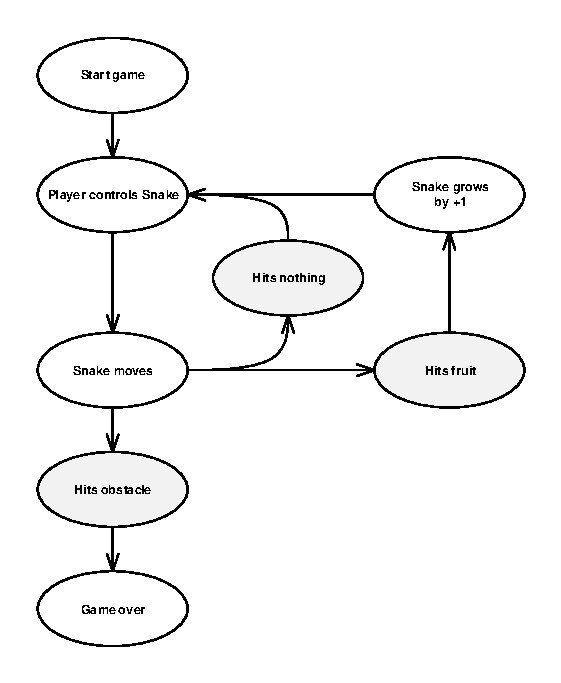
\includegraphics[width=0.5\textwidth, trim={5mm 5mm 5mm 5mm}, clip]{overview/flowgraph}
\caption{Flowchart of basic Snake game}
\label{fig:flow}
\end{figure}

Our game (Snake) is built for the Atmel AVR Mega32 microcontroller. To display the game, we'll use the same type of screen found in the Nokia 3310. To control the game, we have chosen to use a NES controller, where the D-pad (directional pad) is used to direct the Snake.

